\documentclass[12pt]{extarticle}
%Some packages I commonly use.
\usepackage[portuguese]{babel}
\usepackage{graphicx}
\usepackage{framed}
\usepackage[normalem]{ulem}
\usepackage{amsmath}
\usepackage{amsthm}
\usepackage{amssymb}
\usepackage{amsfonts}
\usepackage{enumerate}
\usepackage[utf8]{inputenc}
\usepackage{float}
\usepackage{gensymb}
\usepackage[top=1 in,bottom=1in, left=1 in, right=1 in]{geometry}
\usepackage{multirow}
\usepackage{caption}
\usepackage{subcaption}
\usepackage[utf8]{inputenc}

%A bunch of definitions that make my life easier
\newcommand{\matlab}{{\sc Matlab} }
\newcommand{\cvec}[1]{{\mathbf #1}}
\newcommand{\rvec}[1]{\vec{\mathbf #1}}
\newcommand{\ihat}{\hat{\textbf{\i}}}
\newcommand{\jhat}{\hat{\textbf{\j}}}
\newcommand{\khat}{\hat{\textbf{k}}}
\newcommand{\minor}{{\rm minor}}
\newcommand{\trace}{{\rm trace}}
\newcommand{\spn}{{\rm Span}}
\newcommand{\rem}{{\rm rem}}
\newcommand{\ran}{{\rm range}}
\newcommand{\range}{{\rm range}}
\newcommand{\mdiv}{{\rm div}}
\newcommand{\proj}{{\rm proj}}
\newcommand{\R}{\mathbb{R}}
\newcommand{\N}{\mathbb{N}}
\newcommand{\Q}{\mathbb{Q}}
\newcommand{\Z}{\mathbb{Z}}
\newcommand{\<}{\langle}
\renewcommand{\>}{\rangle}
\renewcommand{\emptyset}{\varnothing}
\newcommand{\attn}[1]{\textbf{#1}}
\theoremstyle{definition}
\newtheorem{theorem}{Theorem}
\newtheorem{corollary}{Corollary}
\newtheorem*{definition}{Definition}
\newtheorem*{example}{Example}
\newtheorem*{note}{Note}
\newtheorem{exercise}{Exercise}
\newcommand{\bproof}{\bigskip {\bf Proof. }}
\newcommand{\eproof}{\hfill\qedsymbol}
\newcommand{\Disp}{\displaystyle}
\newcommand{\qe}{\hfill\(\bigtriangledown\)}
\setlength{\columnseprule}{1 pt}
\usepackage[utf8]{inputenc}

\title{Aula 12 - Eletrodinâmica}
\author{Felipe Salvador}
\date{Atualizado em \today}

\begin{document}

\maketitle

\section{Introdução}
Começamos, agora, a estudar a parte da eletricidade chamada de \textbf{Eletrodinâmica}, que explica o comportamento das cargas em movimentos. Iremos definir quantidades de interesse, além de entender processos elétricos essenciais, que fazem a nossa vida ser bem fácil e tecnológica.

O principal ator dessa parte da teoria é a \textbf{Corrente elétrica (i)} - que é o movimento ordenando de cargas elétricas numa direção. Em especial, o elétron será essa carga em movimento, por causa da sua massa ser bem pequena.

\section{Corrente Elétrica (i)}
A corrente elétrica é definida como: \textbf{Movimento ordenado de cargas elétricas atravessando uma superfície por unidade de tempo.}

\begin{figure}[H]
    \centering
    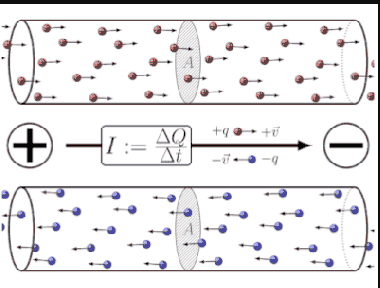
\includegraphics[width=0.6\textwidth]{current.png}
    \caption{Diagrama de como funciona a corrente elétrica. As cargas positivas se movimentam no sentido contrário do que as cargas negativas.}
    \label{fig:current}
\end{figure}

A definição matemática é:
\begin{equation}
    i = \frac{Q}{\Delta t}
\end{equation}
\noindent em que $Q$ é a carga que atravessou a área que eu estou observando e $\Delta t$ é o tempo que eu fiquei observando as cargas atravessarem essa área. Na maioria dos casos, a carga que faz esse trabalho é uma coleção de elétrons. Com isso:
\begin{equation}
    Q = n*\,e
\end{equation}
\noindent em que $n$ é o número de elétrons e $e$ é o valor da carga do elétron $e\approx 1,6.10^{-19}\, C$. Então:
\begin{equation}
    \boxed{i = \frac{n\,e}{\Delta t}}
\end{equation}
Normalmente, o intervalo de tempo observado é de 1s, logo, a corrente elétrica tem a unidade:
\begin{equation}
    [i]=\frac{[C]}{[t]} = A
\end{equation}
\noindent em que $A$ é Ampère, unidade em homenagem à André-Marie Ampère, físico francês, que colaborou muito com os estudos de eletrodinâmica. Essa unidade, então, significa que 1 Ampère é equivalente a dizer que passou uma carga de 1 Coulomb no intervalo de 1 segundo. Vamos descobrir quanto elétrons são necessários para formar uma corrente de 1 Ampère:
\begin{equation}
    1\,A = \frac{n.\,1,6.10^{-19}\,C}{1\, s} \implies n \approx \frac{1.10^{19}}{1,6} \approx 6,25.10^{18}
\end{equation}

Ou seja, para formar uma corrente de 1 A, é necessário ter $6,25.10^{18}$ elétrons passando num intervalo de 1 segundo.

Em geral, não há corrente elétrica espontânea na Natureza. A única forma de fazer uma corrente elétrica é dar algum incentivo a alguma direção para a Natureza, assim as cargas iriam mais facilmente para uma direção, formando a corrente. Esse incentivo é dado a partir de uma \textbf{diferença de potencial elétrico (V) entre 2 pontos, a que chamamos de d.d.p.}. 

Quando temos essa d.d.p., as cargas elétricas num condutor elétrico, são forçadas a se movimentar na direção de menor potencial.

Em geral há 2 tipos de corrente:
\begin{itemize}
    \item \textbf{Corrente contínua} - esse tipo de corrente só flui sentido e, normalmente, o seu valor é constante. Exemplo de uma fonte de corrente contínua é a pilha;
    \item \textbf{Corrente alternada} - a direção e a intensidade da corrente muda ao longo do tempo. Um exemplo de uma fonte de corrente alternada é a tomada 110/220 V.
\end{itemize}

\section{Primeira Lei de Ohm}

Durante o começo dos estudos sobre corrente elétrica, o físico alemão Georg Ohm deduziu uma relação empírica que relacionava 2 grandezas físicas: a corrente elétrica e o potencial elétrico. A relação encontrada é a seguinte:
\begin{equation}
    U = R\,i
\end{equation}
\noindent em que $U$ é a diferença de potencial entre 2 pontos (ex: $U= V_A-V_B$) e $R$ é uma constante chamada de \textbf{resistência elétrica}.

Essa relação conseguiu demonstrar o comportamento e a dependência das 2 quantidades físicas (potencial e corrente). A interpretação dessa relação é que, quando se aplica uma diferença de potencial entre 2 pontos, a corrente que será conduzida dependerá do material em que a corrente caminha. Se o material oferecer mais dificuldade ao movimento das cargas, as cargas vão andar mais lentamente, logo a corrente é menor. Caso contrário, o material incentive o movimento das cargas, as cargas se movimentam rapidamente e, portanto, a corrente elétrica é grande. 

Ela é a equação mais importante para circuitos e iremos tratá-la dela nas próximas aulas.

\section{Potência Elétrica e Efeito Joule}

Uma das formas de saber o quanto de energia elétrica por unidade de tempo um fio está dando é fazendo o cálculo da potência elétrica. Para achar a fórmula, vamos partir da equação do trabalho que uma carga faz num espaço com campo elétrico:
\begin{equation}
    \tau = q\,(V_A-V_B) = q\,U
\end{equation}
\noindent em que 'U' é a diferença de potencial. Sabemos que o trabalho tem unidade de energia (J) e também sabemos que a potência é dada por: $P = E/\Delta t$. Então:
\begin{equation}
    P = \frac{q\,U}{\Delta t}
\end{equation}

Mas, $q/ \Delta t$, pela equação (1), é a definição de corrente elétrica: $i = q/\Delta t$. Logo:
\begin{equation}
    P = U\,i
\end{equation}
\noindent em que a unidade de P é Watt (W). Essa fórmula nos diz sobre o quanto de energia por unidade de tempo as cargas elétricas estão carregando consigo. É por essa fórmula que fazemos os cálculos de potência dos aparelhos elétricos do nosso dia-a-dia. 

Ex: chuveiro elétrico de 4400 W. \textbf{Porque sempre devemos ligar o chuveiro numa fiação de 220V ao invés de 110V?}

Pela fórmula da potência, sabemos que:
\begin{equation}
    P = U\, i \implies 4400 = 220\,i
\end{equation}
Isolando o 'i':
\begin{equation}
    i = \frac{4400}{220} = 20\, A
\end{equation}
Se o chuveiro fosse ligado na fiação de 110 V:
\begin{equation}
    i =\frac{4400}{110} = 40\, A
\end{equation}

A questão aqui é que a corrente duplica de valor e o maior perigo dos equipamentos elétricos é a corrente que passa por ele. \textbf{Correntes elétricas acima de 0,1 A são capazes de matar um ser humano.} Por isso, o ideal é que, para equipamentos elétricos de alta potência (chuveiros, ferros de passar, \textit{airfryer}, grills e chaleiras elétrica), eles sejam da tensão de 220V para que a corrente elétrica seja a menor possível, a fim de evitar acidentes.

Quando uma corrente elétrica passa por qualquer material ou fio, acontece um fenômeno de aquecimento desse material chamado de \textbf{Efeito Joule}. Ele é inerente à eletricidade e acontece devido a dissipação de energia da corrente elétrica no material em forma de energia térmica (aquece o material). É por essa razão que celulares, computadores e qualquer material eletrônico têm que ter um mecanismo de resfriamento para que o seu rendimento de processamento continue alto.
\end{document}
